\begin{figure*}[!t]
  \centering
  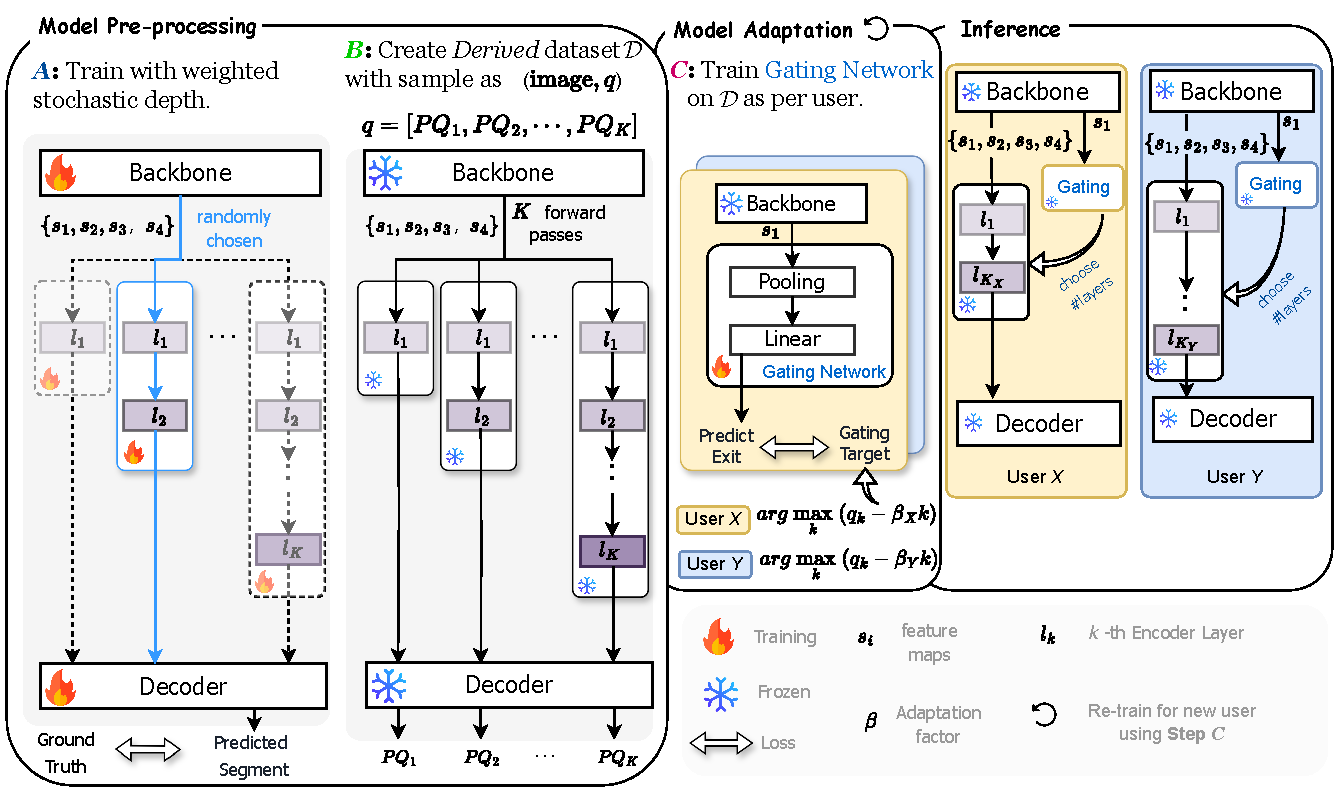
\includegraphics[trim={0 0 1.5em 0},width=\textwidth]{figures/images/main_framework.pdf}
  \caption{\textbf{{\ours} framework.} During the \textit{model pre-processing} phase, we train the model to exit stochastically at $\NGlayer$ potential exits using Step \stepA.  This is followed by Step \stepB, where we use this model to perform inference on the training images at each exit to create a dataset $\train$. In the \textit{model adaptation} phase, we perform Step \stepC to establish a gating target based on the computational budget and train a lightweight gating network. During \textit{inference}, the network adheres to the gating network's output and exits at its designated output layer.}
  \label{fig:main_framework} 
\end{figure*}